%% senseapp_2015.tex
%% V1.3
%% 2007/01/11
%% by Michael Shell
%% See:
%% http://www.michaelshell.org/
%% for current contact information.
%%
%% This is a skeleton file demonstrating the use of IEEEtran.cls
%% (requires IEEEtran.cls version 1.7 or later) with an IEEE conference paper.
%%
%% Support sites:
%% http://www.michaelshell.org/tex/ieeetran/
%% http://www.ctan.org/tex-archive/macros/latex/contrib/IEEEtran/
%% and
%% http://www.ieee.org/

%%*************************************************************************
%% Legal Notice:
%% This code is offered as-is without any warranty either expressed or
%% implied; without even the implied warranty of MERCHANTABILITY or
%% FITNESS FOR A PARTICULAR PURPOSE! 
%% User assumes all risk.
%% In no event shall IEEE or any contributor to this code be liable for
%% any damages or losses, including, but not limited to, incidental,
%% consequential, or any other damages, resulting from the use or misuse
%% of any information contained here.
%%
%% All comments are the opinions of their respective authors and are not
%% necessarily endorsed by the IEEE.
%%
%% This work is distributed under the LaTeX Project Public License (LPPL)
%% ( http://www.latex-project.org/ ) version 1.3, and may be freely used,
%% distributed and modified. A copy of the LPPL, version 1.3, is included
%% in the base LaTeX documentation of all distributions of LaTeX released
%% 2003/12/01 or later.
%% Retain all contribution notices and credits.
%% ** Modified files should be clearly indicated as such, including  **
%% ** renaming them and changing author support contact information. **
%%
%% File list of work: IEEEtran.cls, IEEEtran_HOWTO.pdf, bare_adv.tex,
%%                    bare_conf.tex, bare_jrnl.tex, bare_jrnl_compsoc.tex
%%*************************************************************************

% *** Authors should verify (and, if needed, correct) their LaTeX system  ***
% *** with the testflow diagnostic prior to trusting their LaTeX platform ***
% *** with production work. IEEE's font choices can trigger bugs that do  ***
% *** not appear when using other class files.                            ***
% The testflow support page is at:
% http://www.michaelshell.org/tex/testflow/



% Note that the a4paper option is mainly intended so that authors in
% countries using A4 can easily print to A4 and see how their papers will
% look in print - the typesetting of the document will not typically be
% affected with changes in paper size (but the bottom and side margins will).
% Use the testflow package mentioned above to verify correct handling of
% both paper sizes by the user's LaTeX system.
%
% Also note that the "draftcls" or "draftclsnofoot", not "draft", option
% should be used if it is desired that the figures are to be displayed in
% draft mode.
%
\documentclass[conference]{IEEEtran}
% Add the compsoc option for Computer Society conferences.
%
% If IEEEtran.cls has not been installed into the LaTeX system files,
% manually specify the path to it like:
% \documentclass[conference]{../sty/IEEEtran}


\usepackage[pdftex]{graphicx}
\usepackage{algorithm}
\usepackage{algorithmic}

% Some very useful LaTeX packages include:
% (uncomment the ones you want to load)


% *** MISC UTILITY PACKAGES ***
%
%\usepackage{ifpdf}
% Heiko Oberdiek's ifpdf.sty is very useful if you need conditional
% compilation based on whether the output is pdf or dvi.
% usage:
% \ifpdf
%   % pdf code
% \else
%   % dvi code
% \fi
% The latest version of ifpdf.sty can be obtained from:
% http://www.ctan.org/tex-archive/macros/latex/contrib/oberdiek/
% Also, note that IEEEtran.cls V1.7 and later provides a builtin
% \ifCLASSINFOpdf conditional that works the same way.
% When switching from latex to pdflatex and vice-versa, the compiler may
% have to be run twice to clear warning/error messages.






% *** CITATION PACKAGES ***
%
%\usepackage{cite}
% cite.sty was written by Donald Arseneau
% V1.6 and later of IEEEtran pre-defines the format of the cite.sty package
% \cite{} output to follow that of IEEE. Loading the cite package will
% result in citation numbers being automatically sorted and properly
% "compressed/ranged". e.g., [1], [9], [2], [7], [5], [6] without using
% cite.sty will become [1], [2], [5]--[7], [9] using cite.sty. cite.sty's
% \cite will automatically add leading space, if needed. Use cite.sty's
% noadjust option (cite.sty V3.8 and later) if you want to turn this off.
% cite.sty is already installed on most LaTeX systems. Be sure and use
% version 4.0 (2003-05-27) and later if using hyperref.sty. cite.sty does
% not currently provide for hyperlinked citations.
% The latest version can be obtained at:
% http://www.ctan.org/tex-archive/macros/latex/contrib/cite/
% The documentation is contained in the cite.sty file itself.






% *** GRAPHICS RELATED PACKAGES ***
%
\ifCLASSINFOpdf
  % \usepackage[pdftex]{graphicx}
  % declare the path(s) where your graphic files are
  % \graphicspath{{../pdf/}{../jpeg/}}
  % and their extensions so you won't have to specify these with
  % every instance of \includegraphics
  % \DeclareGraphicsExtensions{.pdf,.jpeg,.png}
\else
  % or other class option (dvipsone, dvipdf, if not using dvips). graphicx
  % will default to the driver specified in the system graphics.cfg if no
  % driver is specified.
  % \usepackage[dvips]{graphicx}
  % declare the path(s) where your graphic files are
  % \graphicspath{{../eps/}}
  % and their extensions so you won't have to specify these with
  % every instance of \includegraphics
  % \DeclareGraphicsExtensions{.eps}
\fi
% graphicx was written by David Carlisle and Sebastian Rahtz. It is
% required if you want graphics, photos, etc. graphicx.sty is already
% installed on most LaTeX systems. The latest version and documentation can
% be obtained at: 
% http://www.ctan.org/tex-archive/macros/latex/required/graphics/
% Another good source of documentation is "Using Imported Graphics in
% LaTeX2e" by Keith Reckdahl which can be found as epslatex.ps or
% epslatex.pdf at: http://www.ctan.org/tex-archive/info/
%
% latex, and pdflatex in dvi mode, support graphics in encapsulated
% postscript (.eps) format. pdflatex in pdf mode supports graphics
% in .pdf, .jpeg, .png and .mps (metapost) formats. Users should ensure
% that all non-photo figures use a vector format (.eps, .pdf, .mps) and
% not a bitmapped formats (.jpeg, .png). IEEE frowns on bitmapped formats
% which can result in "jaggedy"/blurry rendering of lines and letters as
% well as large increases in file sizes.
%
% You can find documentation about the pdfTeX application at:
% http://www.tug.org/applications/pdftex





% *** MATH PACKAGES ***
%
%\usepackage[cmex10]{amsmath}
% A popular package from the American Mathematical Society that provides
% many useful and powerful commands for dealing with mathematics. If using
% it, be sure to load this package with the cmex10 option to ensure that
% only type 1 fonts will utilized at all point sizes. Without this option,
% it is possible that some math symbols, particularly those within
% footnotes, will be rendered in bitmap form which will result in a
% document that can not be IEEE Xplore compliant!
%
% Also, note that the amsmath package sets \interdisplaylinepenalty to 10000
% thus preventing page breaks from occurring within multiline equations. Use:
%\interdisplaylinepenalty=2500
% after loading amsmath to restore such page breaks as IEEEtran.cls normally
% does. amsmath.sty is already installed on most LaTeX systems. The latest
% version and documentation can be obtained at:
% http://www.ctan.org/tex-archive/macros/latex/required/amslatex/math/





% *** SPECIALIZED LIST PACKAGES ***
%
%\usepackage{algorithmic}
% algorithmic.sty was written by Peter Williams and Rogerio Brito.
% This package provides an algorithmic environment fo describing algorithms.
% You can use the algorithmic environment in-text or within a figure
% environment to provide for a floating algorithm. Do NOT use the algorithm
% floating environment provided by algorithm.sty (by the same authors) or
% algorithm2e.sty (by Christophe Fiorio) as IEEE does not use dedicated
% algorithm float types and packages that provide these will not provide
% correct IEEE style captions. The latest version and documentation of
% algorithmic.sty can be obtained at:
% http://www.ctan.org/tex-archive/macros/latex/contrib/algorithms/
% There is also a support site at:
% http://algorithms.berlios.de/index.html
% Also of interest may be the (relatively newer and more customizable)
% algorithmicx.sty package by Szasz Janos:
% http://www.ctan.org/tex-archive/macros/latex/contrib/algorithmicx/




% *** ALIGNMENT PACKAGES ***
%
%\usepackage{array}
% Frank Mittelbach's and David Carlisle's array.sty patches and improves
% the standard LaTeX2e array and tabular environments to provide better
% appearance and additional user controls. As the default LaTeX2e table
% generation code is lacking to the point of almost being broken with
% respect to the quality of the end results, all users are strongly
% advised to use an enhanced (at the very least that provided by array.sty)
% set of table tools. array.sty is already installed on most systems. The
% latest version and documentation can be obtained at:
% http://www.ctan.org/tex-archive/macros/latex/required/tools/


%\usepackage{mdwmath}
%\usepackage{mdwtab}
% Also highly recommended is Mark Wooding's extremely powerful MDW tools,
% especially mdwmath.sty and mdwtab.sty which are used to format equations
% and tables, respectively. The MDWtools set is already installed on most
% LaTeX systems. The lastest version and documentation is available at:
% http://www.ctan.org/tex-archive/macros/latex/contrib/mdwtools/


% IEEEtran contains the IEEEeqnarray family of commands that can be used to
% generate multiline equations as well as matrices, tables, etc., of high
% quality.


%\usepackage{eqparbox}
% Also of notable interest is Scott Pakin's eqparbox package for creating
% (automatically sized) equal width boxes - aka "natural width parboxes".
% Available at:
% http://www.ctan.org/tex-archive/macros/latex/contrib/eqparbox/





% *** SUBFIGURE PACKAGES ***
%\usepackage[tight,footnotesize]{subfigure}
% subfigure.sty was written by Steven Douglas Cochran. This package makes it
% easy to put subfigures in your figures. e.g., "Figure 1a and 1b". For IEEE
% work, it is a good idea to load it with the tight package option to reduce
% the amount of white space around the subfigures. subfigure.sty is already
% installed on most LaTeX systems. The latest version and documentation can
% be obtained at:
% http://www.ctan.org/tex-archive/obsolete/macros/latex/contrib/subfigure/
% subfigure.sty has been superceeded by subfig.sty.



%\usepackage[caption=false]{caption}
%\usepackage[font=footnotesize]{subfig}
% subfig.sty, also written by Steven Douglas Cochran, is the modern
% replacement for subfigure.sty. However, subfig.sty requires and
% automatically loads Axel Sommerfeldt's caption.sty which will override
% IEEEtran.cls handling of captions and this will result in nonIEEE style
% figure/table captions. To prevent this problem, be sure and preload
% caption.sty with its "caption=false" package option. This is will preserve
% IEEEtran.cls handing of captions. Version 1.3 (2005/06/28) and later 
% (recommended due to many improvements over 1.2) of subfig.sty supports
% the caption=false option directly:
%\usepackage[caption=false,font=footnotesize]{subfig}
%
% The latest version and documentation can be obtained at:
% http://www.ctan.org/tex-archive/macros/latex/contrib/subfig/
% The latest version and documentation of caption.sty can be obtained at:
% http://www.ctan.org/tex-archive/macros/latex/contrib/caption/




% *** FLOAT PACKAGES ***
%
%\usepackage{fixltx2e}
% fixltx2e, the successor to the earlier fix2col.sty, was written by
% Frank Mittelbach and David Carlisle. This package corrects a few problems
% in the LaTeX2e kernel, the most notable of which is that in current
% LaTeX2e releases, the ordering of single and double column floats is not
% guaranteed to be preserved. Thus, an unpatched LaTeX2e can allow a
% single column figure to be placed prior to an earlier double column
% figure. The latest version and documentation can be found at:
% http://www.ctan.org/tex-archive/macros/latex/base/



%\usepackage{stfloats}
% stfloats.sty was written by Sigitas Tolusis. This package gives LaTeX2e
% the ability to do double column floats at the bottom of the page as well
% as the top. (e.g., "\begin{figure*}[!b]" is not normally possible in
% LaTeX2e). It also provides a command:
%\fnbelowfloat
% to enable the placement of footnotes below bottom floats (the standard
% LaTeX2e kernel puts them above bottom floats). This is an invasive package
% which rewrites many portions of the LaTeX2e float routines. It may not work
% with other packages that modify the LaTeX2e float routines. The latest
% version and documentation can be obtained at:
% http://www.ctan.org/tex-archive/macros/latex/contrib/sttools/
% Documentation is contained in the stfloats.sty comments as well as in the
% presfull.pdf file. Do not use the stfloats baselinefloat ability as IEEE
% does not allow \baselineskip to stretch. Authors submitting work to the
% IEEE should note that IEEE rarely uses double column equations and
% that authors should try to avoid such use. Do not be tempted to use the
% cuted.sty or midfloat.sty packages (also by Sigitas Tolusis) as IEEE does
% not format its papers in such ways.





% *** PDF, URL AND HYPERLINK PACKAGES ***
%
%\usepackage{url}
% url.sty was written by Donald Arseneau. It provides better support for
% handling and breaking URLs. url.sty is already installed on most LaTeX
% systems. The latest version can be obtained at:
% http://www.ctan.org/tex-archive/macros/latex/contrib/misc/
% Read the url.sty source comments for usage information. Basically,
% \url{my_url_here}.





% *** Do not adjust lengths that control margins, column widths, etc. ***
% *** Do not use packages that alter fonts (such as pslatex).         ***
% There should be no need to do such things with IEEEtran.cls V1.6 and later.
% (Unless specifically asked to do so by the journal or conference you plan
% to submit to, of course. )


% correct bad hyphenation here
\hyphenation{op-tical net-works semi-conduc-tor}


\begin{document}
%
% paper title
% can use linebreaks \\ within to get better formatting as desired
\title{Multichannel RPL Variant}


% author names and affiliations
% use a multiple column layout for up to three different
% affiliations
\author{\IEEEauthorblockN{Noradila Nordin}
\IEEEauthorblockA{
University College London\\
%Electronic and Electrical Engineering Department\\ University College London\\ 
%London, WC1E 7JE\\
Email: noradila.nordin.12@ucl.ac.uk}
\and
\IEEEauthorblockN{Richard G Clegg}
\IEEEauthorblockA{Imperial College London\\
Email: richard@richardclegg.org}
\and
\IEEEauthorblockN{Miguel Rio}
\IEEEauthorblockA{University College London\\
Email: miguel.rio@ucl.ac.uk}}

% conference papers do not typically use \thanks and this command
% is locked out in conference mode. If really needed, such as for
% the acknowledgment of grants, issue a \IEEEoverridecommandlockouts
% after \documentclass

% for over three affiliations, or if they all won't fit within the width
% of the page, use this alternative format:
% 
%\author{\IEEEauthorblockN{Michael Shell\IEEEauthorrefmark{1},
%Homer Simpson\IEEEauthorrefmark{2},
%James Kirk\IEEEauthorrefmark{3}, 
%Montgomery Scott\IEEEauthorrefmark{3} and
%Eldon Tyrell\IEEEauthorrefmark{4}}
%\IEEEauthorblockA{\IEEEauthorrefmark{1}School of Electrical and Computer Engineering\\
%Georgia Institute of Technology,
%Atlanta, Georgia 30332--0250\\ Email: see http://www.michaelshell.org/contact.html}
%\IEEEauthorblockA{\IEEEauthorrefmark{2}Twentieth Century Fox, Springfield, USA\\
%Email: homer@thesimpsons.com}
%\IEEEauthorblockA{\IEEEauthorrefmark{3}Starfleet Academy, San Francisco, California 96678-2391\\
%Telephone: (800) 555--1212, Fax: (888) 555--1212}
%\IEEEauthorblockA{\IEEEauthorrefmark{4}Tyrell Inc., 123 Replicant Street, Los Angeles, California 90210--4321}}




% use for special paper notices
%\IEEEspecialpapernotice{(Invited Paper)}




% make the title area
\maketitle


\begin{abstract}
%\boldmath
%The abstract goes here.
This paper proposes a new multi-channel tree building protocol for ad-hoc sensor networks. Our protocol alleviates the effect of interference which results in improved network efficiency and stability, link reliability and minimised latency. 
        Our proposal takes into account all available channels to utilise the spectrum. It checks the condition of all the channels before deciding on a channel to switch into. The successful transmission rate of the channels are stored externally from the sensors which can be accessed when require. This information is used to limit the channels to be considered when channel switching is invoked. The channel that is selected is checked for any changes in its condition that might had taken place after it was checked previously before committing to the channel. The results and decisions are informed to the other nodes to update their neighbour table. We use two-hop colouring protocol to avoid collision. 
	Our protocol is inspired by the routing protocol for low power and lossy networks (RPL). Packets will be sent to the destination the same way as a single channel RPL but with less loss. 
	All nodes are battery operated except for the low power border route (LPBR). This enables a centralised channel switching process at the LPBR. The channel switching process take place after the topology is formed to further improve the transmission rate on the best paths.
	We implement and evaluate our solution using the Contiki framework. Our experimental results demonstrate an increased resilience to interference, and significant higher throughput making better use of the total available spectrum and link stability. 

\end{abstract}
% IEEEtran.cls defaults to using nonbold math in the Abstract.
% This preserves the distinction between vectors and scalars. However,
% if the conference you are submitting to favors bold math in the abstract,
% then you can use LaTeX's standard command \boldmath at the very start
% of the abstract to achieve this. Many IEEE journals/conferences frown on
% math in the abstract anyway.

% no keywords




% For peer review papers, you can put extra information on the cover
% page as needed:
% \ifCLASSOPTIONpeerreview
% \begin{center} \bfseries EDICS Category: 3-BBND \end{center}
% \fi
%
% For peerreview papers, this IEEEtran command inserts a page break and
% creates the second title. It will be ignored for other modes.
\IEEEpeerreviewmaketitle

\section{Introduction}
\label{sec:introduction}
///add intro - comment and why it is an important topic

%challenges and solution
Sensor networks have to contend with an increasing number of devices that cause wireless interference. Organising the network topology around this interference becomes an enabler for increasing transmission efficiency at a smaller energy cost. Wireless Sensor Networks (WSN) typically use low power radios such as IEEE 802.15.4, a relatively short range transmission standard radio technology in the 2.4Ghz band. The standard allows transmission to occur on several different channels within this band.  Unfortunately, the channels used by this technology often suffer interference, for example, from WiFi and Bluetooth. WSNs need to be able to operate reliably in the presence of such interference.  

%highlight of existing solutions and limitation (remove details!)
Multichannel communication in wireless networks can alleviate the effects of interference which, as a result, can improve the network efficiency and stability, link reliability and minimise latency. It also enables communication between physically proximate nodes to occur simultaneously without the risk of collision if the communicating nodes use different channels. However, not all channels are free from interference; thus, there is a need to hop to another channel when the quality of the channel deteriorates. Two commonly used types of channel hopping \cite{watteyne} are blind channel hopping and whitelisting. In blind channel hopping, nodes choose from all available channels. Whitelisting on the other hand, filters out those channels that may have bad interference properties. Many studies make use of channel whitelisting such as in \cite{watteyne}, \cite{wu}, Chrysso \cite{chrysso} and MiCMAC \cite{micmac}. However, they used different channels with channel 26 in common in their respective experiments. 
%Many studies make use of channel whitelisting such as \cite{watteyne} which claimed that channels 11, 15, 25 and 26 are free from Wi-Fi \cite{wu}. Chrysso \cite{chrysso} uses channel 11, 14, 20, 22 and 26, and MiCMAC \cite{micmac} uses channel 15, 20, 25 and 26 in their respective experiments. 
It is notable that these protocols can use all available channels without whitelisting. However, they do not have a mechanism to check the channel condition before using it for packet transmission. %In \cite{micmac}, MiCMAC sees its performance degraded when using more than 4 channels, thus the decision on specifying 4 channels to be included in their experiment. 
MiCMAC uses different wakeup channel each time it wakes up, thus, it sends packet on different channel each time. However, it might try to send on bad channels for a while before it finds a good channel to deliver the packet. Chrysso on the other hand, switches the affected nodes to a new set of channels upon detecting interference. It would require frequent channel switching if all channels are to be considered.

It is clear that it is impossible to find a single channel guaranteed free from interference and there is no consensus on the best channel to use. Our work takes into account all available channels to utilise the spectrum and checks the condition of the channels before hopping to avoid those channels with interference.

Several previous studies have developed a multichannel MAC layer but, despite the potential benefits none are yet widely implemented in real world deployments. The usual focus is on MAC layers that operate in an autonomous fashion. This paper focuses instead on a Multichannel Cross-Layer Routing Protocol (MCRP) which allows a centralised intelligence to make and communicate decisions about channels and this decision is implemented by the MAC layer. MCRP provides feedback when a channel is subject to interference using a probing phase. This protocol is tested using a two-hop colouring protocol to reduce interference between physically proximate nodes trying to communicate on the same channel. The system is failed safe in the sense that the WSN functions if the central system which assigns channels fails temporarily or permanently.

%which allows a centralised intelligence to determine which channels each node. The protocol also introduces a probing phase that checks whether assigned channels are free of interference. This protocol is tested using a two-hop colouring protocol to reduce interference between physically proximate nodes trying to communicate on the same channel. The system is failed safe in the sense that the WSN functions if the central system which assigns channels fails temporarily or permanently.

%This paper focuses instead on a cross-layer multi-channel model where a centralised controller can make and communicate decisions about channels and this decision is implemented by the MAC layer. Our Multichannel Cross-Layer Routing Protocol (MCRP) provides feedback when a channel is subject to interference using a probing phase.

%The nodes are given different channels by a centralised controller behind the Low Power Border Router (LPBR). This means that the mechanism for assigning nodes to channels can be aware of the entire topology and can use more advanced algorithms to choose which channels are assigned to which nodes. Nodes are given a listening channel and their neighbours must send to them on that channel. In other words, a node listens on a single channel but sends on many channels. This enables communication between several sender-intermediate nodes towards the LPBR to occur simultaneously in a collision free manner.

%how the proposed work and their limitation - our contribution
%The IETF standard IPv6 Routing Protocol for Low-Power and Lossy Networks (RPL) is a routing protocol for WSN that allows nodes to self-organise a communicating network of neighbouring nodes. 

%In this paper, we develop a cross-layer multi-channel protocol which allows a centralised intelligence to determine which channels each node. The protocol also introduces a probing phase that checks whether assigned channels are free of interference. This protocol is tested using a two-hop colouring protocol to reduce interference between physically proximate nodes trying to communicate on the same channel. The system is failed safe in the sense that the WSN functions if the central system which assigns channels fails temporarily or permanently.

We implement MCRP in Contiki and evaluate the protocol in Cooja simulated environment and in 26-nodes testbed FlockLab \cite{flocklab}. We demonstrate that MCRP avoids channels with interference which greatly reduces the effects of interference on the network.

%The nodes run on IPv6 and use RPL as the routing protocol; to demonstrate that MCRP channel changes do not intervene with RPL protocol and the network is fully functional during our protocol's channel changes.



%The IETF standard IPv6 Routing Protocol for Low-Power and Lossy Networks (RPL) is a routing protocol for WSN that allows nodes to self-organise a communicating network of neighbouring nodes. In this paper, we develop a cross-layer multi-channel protocol which allows a centralised intelligence to determine which channels each node should listen on and ensures that their neighbours send on the correct channel. The protocol also introduces a probing phase that checks whether assigned channels are free of interference. This protocol is tested using a two-hop colouring protocol that ensures nodes located within two hops of each other in the network are listening on different channels (that should reduce interference between physically proximate nodes trying to communicate on the same channel).  The system is failed safe in the sense that the WSN functions if the central system which assigns channels fails temporarily or permanently.

%The control messages are sent to the nodes on their usual listening channel as a unicast which eliminates the need for a separate control channel. The changes of channel occur after the RPL topology set up phase. We show that this allows the network to avoid channels with interference and we demonstrate in simulation that this greatly reduces the effects of interference. While our protocol has an overhead in terms of packets sent and in terms of set up time, the number of packets sent is still low overall and during the multi-channel set up phase the system is still capable of sending traffic, thus the network is still fully functional after RPL set up and during our protocol's channel changes.

The rest of the paper is organised as follows: Section \ref{sec:relatedwork} presents related work to multichannel protocols. Section \ref{sec:multichannel} describes the key idea of our proposed protocol and the high-level design and the implementation of the protocol in Contiki. We describe and evaluate the experimental results in Section \ref{sec:evaluation}. Finally, we conclude in Section \ref{sec:conclusion}.


%\section{Introduction}
% no \IEEEPARstart
%This demo file is intended to serve as a ``starter file''
%for IEEE conference papers produced under \LaTeX\ using
%IEEEtran.cls version 1.7 and later.
% You must have at least 2 lines in the paragraph with the drop letter
% (should never be an issue)
%I wish you the best of success.

%\hfill mds
 
%\hfill January 11, 2007

%\subsection{Subsection Heading Here}
%Subsection text here.


%\subsubsection{Subsubsection Heading Here}
%Subsubsection text here.


% An example of a floating figure using the graphicx package.
% Note that \label must occur AFTER (or within) \caption.
% For figures, \caption should occur after the \includegraphics.
% Note that IEEEtran v1.7 and later has special internal code that
% is designed to preserve the operation of \label within \caption
% even when the captionsoff option is in effect. However, because
% of issues like this, it may be the safest practice to put all your
% \label just after \caption rather than within \caption{}.
%
% Reminder: the "draftcls" or "draftclsnofoot", not "draft", class
% option should be used if it is desired that the figures are to be
% displayed while in draft mode.
%
%\begin{figure}[!t]
%\centering
%\includegraphics[width=2.5in]{myfigure}
% where an .eps filename suffix will be assumed under latex, 
% and a .pdf suffix will be assumed for pdflatex; or what has been declared
% via \DeclareGraphicsExtensions.
%\caption{Simulation Results}
%\label{fig_sim}
%\end{figure}

% Note that IEEE typically puts floats only at the top, even when this
% results in a large percentage of a column being occupied by floats.


% An example of a double column floating figure using two subfigures.
% (The subfig.sty package must be loaded for this to work.)
% The subfigure \label commands are set within each subfloat command, the
% \label for the overall figure must come after \caption.
% \hfil must be used as a separator to get equal spacing.
% The subfigure.sty package works much the same way, except \subfigure is
% used instead of \subfloat.
%
%\begin{figure*}[!t]
%\centerline{\subfloat[Case I]\includegraphics[width=2.5in]{subfigcase1}%
%\label{fig_first_case}}
%\hfil
%\subfloat[Case II]{\includegraphics[width=2.5in]{subfigcase2}%
%\label{fig_second_case}}}
%\caption{Simulation results}
%\label{fig_sim}
%\end{figure*}
%
% Note that often IEEE papers with subfigures do not employ subfigure
% captions (using the optional argument to \subfloat), but instead will
% reference/describe all of them (a), (b), etc., within the main caption.


% An example of a floating table. Note that, for IEEE style tables, the 
% \caption command should come BEFORE the table. Table text will default to
% \footnotesize as IEEE normally uses this smaller font for tables.
% The \label must come after \caption as always.
%
%\begin{table}[!t]
%% increase table row spacing, adjust to taste
%\renewcommand{\arraystretch}{1.3}
% if using array.sty, it might be a good idea to tweak the value of
% \extrarowheight as needed to properly center the text within the cells
%\caption{An Example of a Table}
%\label{table_example}
%\centering
%% Some packages, such as MDW tools, offer better commands for making tables
%% than the plain LaTeX2e tabular which is used here.
%\begin{tabular}{|c||c|}
%\hline
%One & Two\\
%\hline
%Three & Four\\
%\hline
%\end{tabular}
%\end{table}


% Note that IEEE does not put floats in the very first column - or typically
% anywhere on the first page for that matter. Also, in-text middle ("here")
% positioning is not used. Most IEEE journals/conferences use top floats
% exclusively. Note that, LaTeX2e, unlike IEEE journals/conferences, places
% footnotes above bottom floats. This can be corrected via the \fnbelowfloat
% command of the stfloats package.

\section{Related Work}
\label{sec:relatedwork}

\section{Multichannel Cross-Layer Routing Protocol}
\label{sec:multichannel}

Multichannel Cross-Layer Routing Protocol (MCRP) concentrates on finding channels for nodes that are
free from or have low interference. It allows the allocation of these channels in a way likely
to minimise the chances of nodes which are physically near communicating on the same channel and
hence reduce cross interference between different pairs of nodes.

\subsection{Overview}

%\explain the ideas (state machine?), reasons for doing

The design of the multichannel protocol is based on several crucial observations:
\begin{itemize}
\item Channel assignment - Sensors have limited memory and battery capabilities. In order to maximise the sensors lifetime, a centralised LPBR that has larger memory and fully powered is used for decision making. LPBR has a complete knowledge of the topology which enables it to make good channel assignment decisions based on the criteria that are explained in the next section. 
%LPBR assigns channel to the nodes.
%This centralised processes at the LPBR enable the other nodes that are battery powered to minimise the use of the energy in packets transmission. LPBR is fully powered which is the main reason for placing intelligence on it.
%LPBR keeps track of the channel conditions based on the feedback it receives from the nodes. All intelligence is done at LPBR.
%by considering load balancing in channels.
\item Interference - External interference cannot be predicted, thus channels cannot be allocated beforehand as it varies over time and locations. It is impossible to determine a single channel that is free from interference at any location. Our protocol checks the channel condition each time before deciding on a channel change to reduce interference and maximise throughput.
\item Frequency diversity - RPL is typically used with ContikiMAC which is a single channel protocol. By using multichannel, we increase the robustness of the network towards interference. However, applying multichannel to the existing RPL may hinder neighbour detection and RPL processes to maintain the network topology as it does not switch to the correct channel. We overcome this problem by enabling unicast in neighbour detection and RPL control messages. %We assume that no new nodes should join the topology after the initial setup.
%we need to ensure the node knows the correct channel to reach the neighbours. RPL forms and maintains the network topology through its control messages. Applying multichannel to the existing RPL may hinder neighbour detection and RPL processes and it does not have any means of switching to the correct channel. 
\end{itemize}

Our cross-layer multi-channel protocol focuses on the network and application layer of the protocol. This allows channel assignment decisions to be made thoroughly without being limited by the low layer complexity. The channel assignment processes take place only after the topology tree has been formed by RPL and stabilised. The system
has two parts: a central algorithm which can be collocated with the LPBR and selects which channel each node should listen on; and a protocol which allows the network to communicate the channel change decision, probe the new channel and either communicate the success of the change or fall back to the previous channel. 

%Figure 1 shows the design of Multichannel RPL. The states are explained in the next sections.

%\begin{figure}
%\centering
%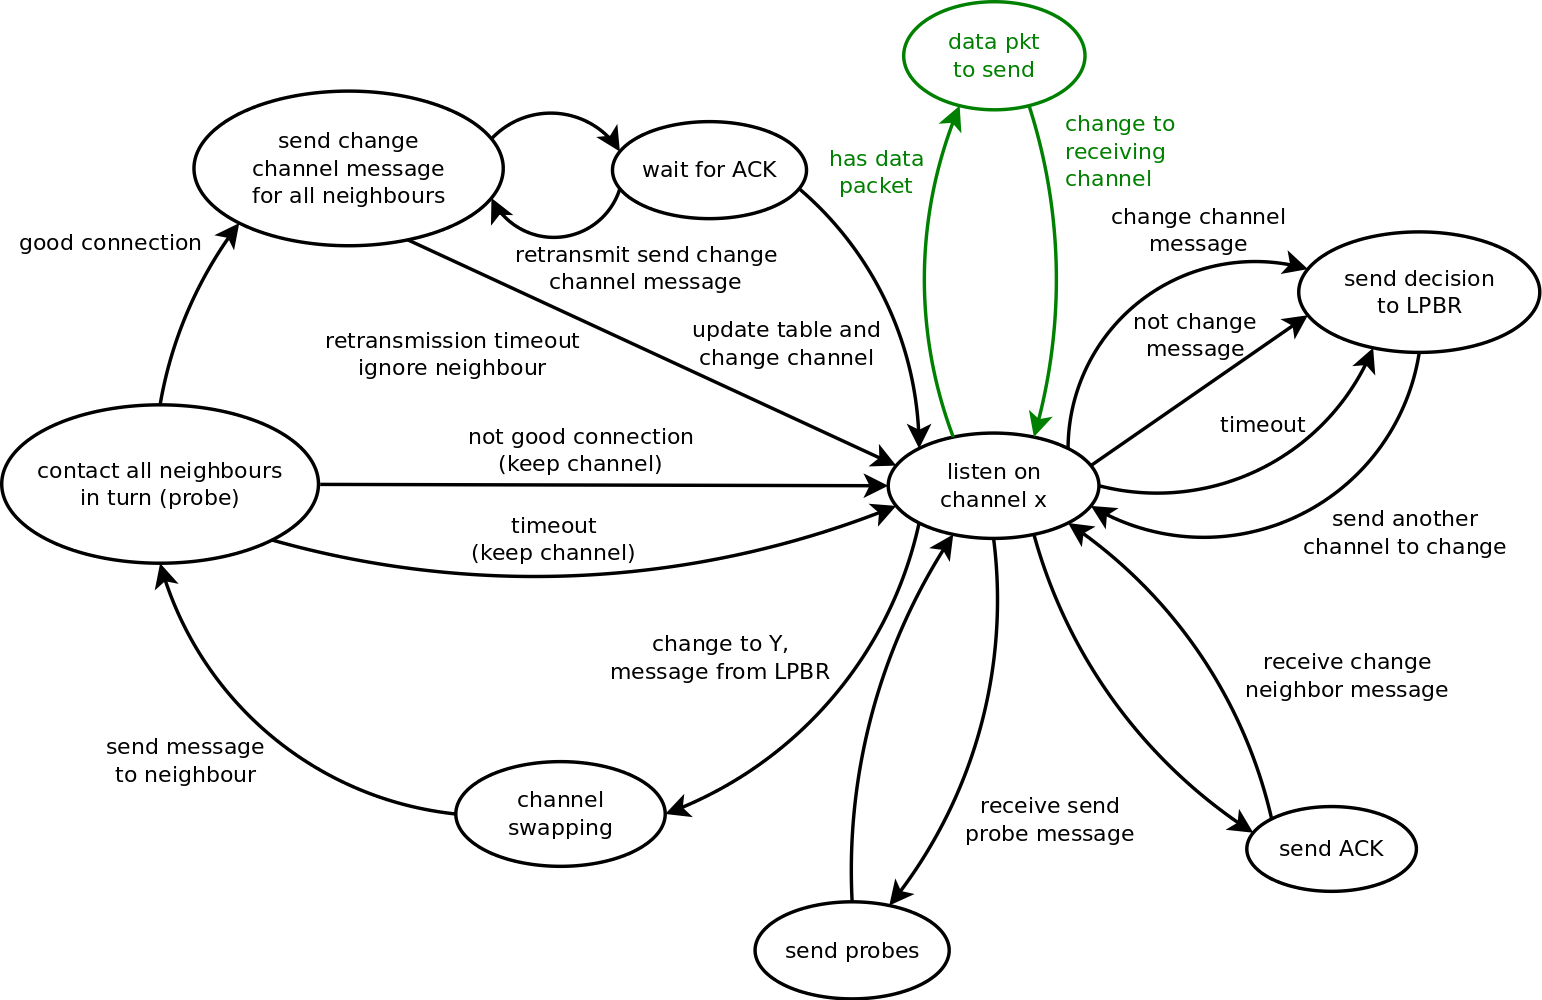
\includegraphics[height=7.2cm]{stateDiagram}
%\caption{State machine for channel switching.}
%\label{fig:example}
%\end{figure}

\subsection{Channel Selection Strategy}

%//LPBR decides the channel; random at first (or maybe not) and then based on probing that were done previously stating the condition of channels.
%//be more detail - better description of 2-hop strategy reasoning. %WHY?? keep them not to interference so much with each other
The system we propose is general and any algorithm can be used at the LPBR to assign channels. In this paper we
use a two-hop colouring protocol to select a channel to be assigned to a node. Channels are chosen in a way that
ensures no nodes within two hops of each other on the network are listening on the same channel.
This allows fair load balancing on the channels and reduces channel interference that could occur when two nearby nodes transmit together on the same channel. The nodes used in this paper have a transmission range of approximately 50 metres indoors and 125 metres outdoors. It could be the case, therefore, that many nodes in a sensor network are in the transmission range of each other and potentially interfered with.

As in standard RPL all nodes are initialised to channel 26 by default. The usual RPL set up mechanism is used to exchange control messages that are required to form an optimised topology before channel assignments can take place. The nodes will only be on the same channel once during the initial setup. Channel 26 is chosen as this is the usual RPL default initial channel since it often has fewer interference problems with WiFi and other sources. The studies in \cite{chrysso}\cite{micmac}\cite{watteyne} use several channels in their experiments and have channel 26 in common.
	
%**TWO HOP COLOURING STRATEGY?
%\subsubsection{Two Hops Neighbour Strategy -}


%//how it works?
%During the initial setup, LPBR does not have any knowledge of the channels condition. All channels are assumed to be available to be used. LPBR assigns a random channel to a node. The node that receives the channel change message will inform all of its neighbour of its new channel. The neighbours will update their neighbour table to hold the new channel value as the node current channel for transmission. The neighbour nodes will in turn, send probing messages.

\iffalse
\begin{algorithm}
\caption{Two hops neighbour strategy}
\begin{algorithmic} 
\STATE $newChannel \neq currentChannel$
\STATE $newChannel \leftarrow x$

\REQUIRE\emph{first hop}{}:
\WHILE {$retry \neq 4$}
\IF{$node = LPBRneighbour$}

\IF {$newChannel \neq LPBRChannel$}
\STATE {\emph {second hop}}
\ELSE
\STATE $newChannel \leftarrow y$
\ENDIF

\ELSE [$node = neighbourNeighbour$]
\IF {$newChannel \neq neighbourChannel$}
\STATE {\emph {second hop}}
\ELSE
\STATE $newChannel \leftarrow y$
\ENDIF
\ENDIF
\ENDWHILE


\REQUIRE\emph{second hop}{}:
\WHILE {$retry \neq 4$}
\IF{$node = LPBRneighbour$}

\IF {$newChannel \neq LPBRneighboursChannel$}
\STATE $newChannel \leftarrow OK$
\ELSE
\STATE $newChannel \leftarrow y$
\ENDIF

\ELSE [$node = neighbourNeighbour$]
\IF {$newChannel \neq neighbourNeighboursChannel$}
\STATE $newChannel \leftarrow OK$
\ELSE
\STATE $newChannel \leftarrow y$
\ENDIF
\ENDIF
\ENDWHILE
\end{algorithmic}
\end{algorithm}
\fi

In the two-hop colouring algorithm, the LPBR chooses a node to which it will assign a channel to listen on.  
This selection is random from channels 11 to 26 (the full range available). The algorithm checks neighbours and neighbours of neighbours to see if any of those are listening on this channel already. If any are, a new channel is picked from the remaining list of available channels. If the LPBR has knowledge of existing bad channels then those channels can be black listed.  Knowledge of channel interference (gained by probing, see later description) can be used to decide that a channel should not be used. If a channel is found then the channel switching protocol is used (see section \ref{sec:channelswitch}). If no channel can be found meeting these conditions the current
channel is kept.  

The node selection algorithm must only attempt one channel change at a time. The protocol ensures that the
channel change attempt will always result in a message returned to the LPBR either confirming the new channel
or announcing a reversion to the old channel. Until one or other of these happens no new channel change will
be made.

%***probing tries to avoid the interference channel.


%We could increase the number of probing messages by increasing the buffer size or the radio duty cycle (to be confirmed!!) but we chosen not to because increasing buffer size means that we will be using more memory which is not practical as we have limited memory available. If we increase the radio duty cycle, that would cost us more energy as the node will be awake more frequent and the nodes will not be in sync as they would have different radio duty cycle. That would increase the chance of packet loss. Our other option is to run the probing for a longer time.

%////FUTURE WORK?
%Even though external interference varies over time, it is unlikely that the channel quality fluctuates frequently within minutes that would affect the receiving success rate. Thus, the channel quality check is invoke on three (cases? situations?); on initialisation, when receiving LPBR channel change message and when the packet delivery ratio (PDR) drops. ***NOT SURE  


%****
%Each node keeps the counter of packets it has sent and received. It will send the information to LPBR periodically in order for LPBR to get a full view on the condition of the channels. LPBR will then decide if the node needs to change to another channel depending on the sent and received information. If the node does not perform well based on the number of received packets less than the number of packets being sent, LPBR will decide on a new channel the node needs to change into. The node will go through the channel changing processes to decide if the new channel is performing better than the previous channel before (settling?) for the new channel.

\subsection{Channel Switching}
\label{sec:channelswitch}

%//explain LPBR that decides whether the nodes should stay on the same channel or switch to a new channel based on the information it gathers through nodes probing.

%State machine explanation should be here?

\begin{figure}
\centering
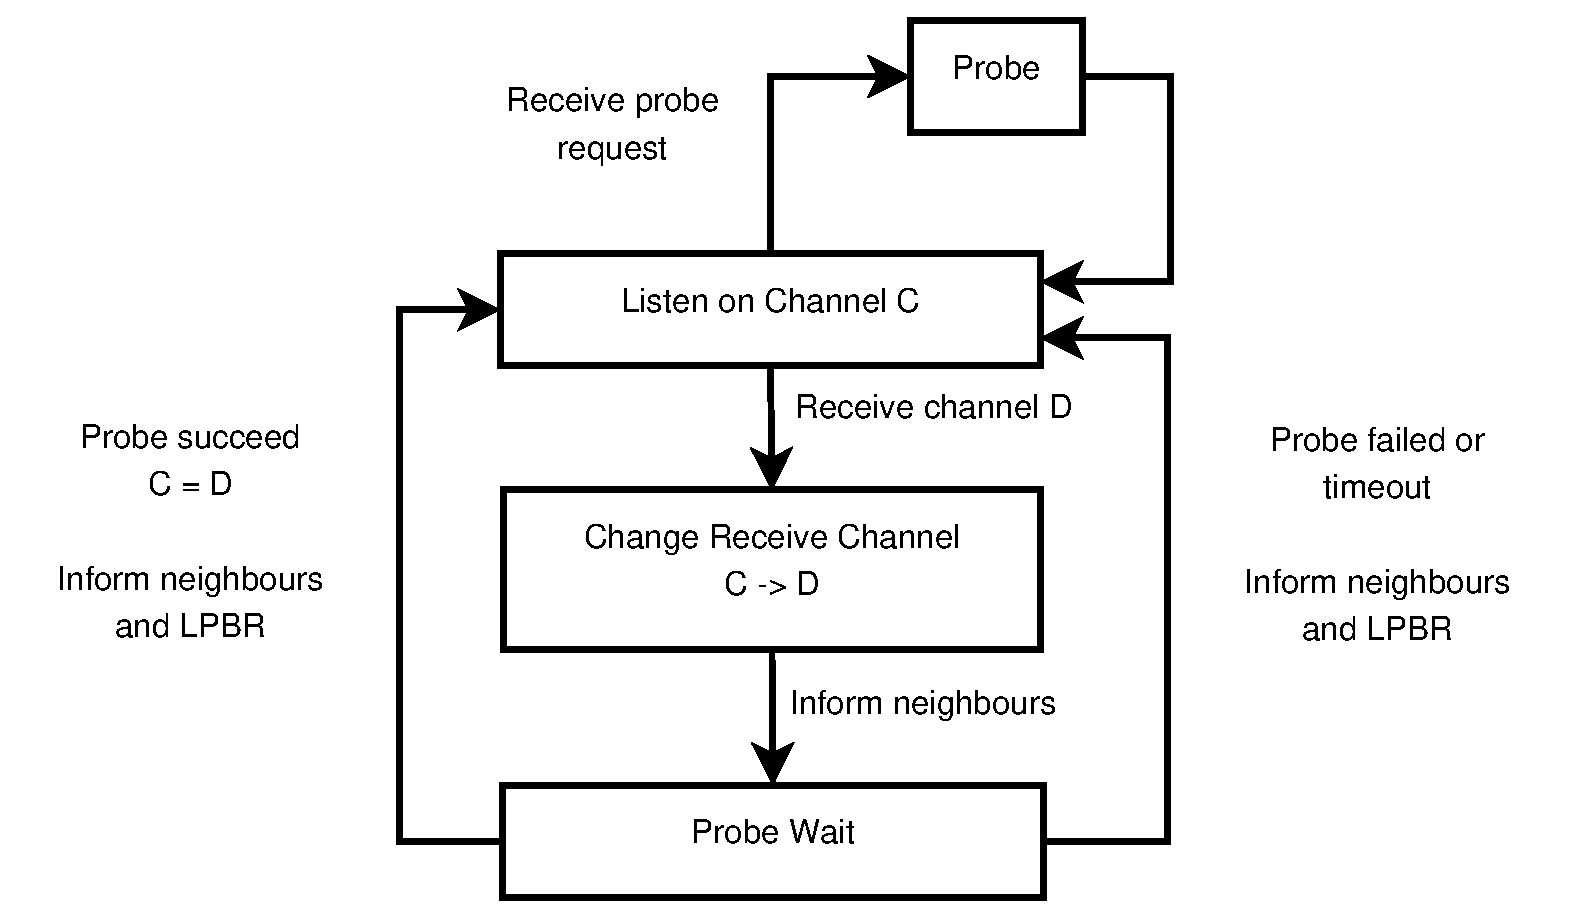
\includegraphics[width=3.5in]{Diagram1.eps}
\caption{Channel switching processes}
\label{fig_sim}
\end{figure}

Figure \ref{fig_sim} shows the state machine for the channel switching protocol.
As explained in the previous section, a choice of a new channel by the channel selection algorithm causes a change channel message to be sent to the appropriate node. 
On receiving a channel change message a node $N$ stores its current channel $C$ and communicates to all its neighbours the new channel $D$ it wishes to change to.  Those neighbours will update their neighbour tables to ensure that they now send to node $N$ on channel $D$.  The node $N$ now begins the channel quality checking process (see section \ref{sec:channelquality} with each neighbour in turn by sending them a probe request.  If this process fails for any neighbour then the node reverts to channel $C$.  Node $N$ informs its neighbours of this reversion to channel $C$ and informs the LPBR of the channel checking results and its reversion to listening on channel $C$. If all channel quality checks succeed the node $N$. It is important to emphasise that the network remains fully functional and connected at all stages of this protocol (however, the channel checking process uses probe packets that might interfere with other transmissions temporarily).

\subsection{Channel Quality Checking}
\label{sec:channelquality}
%channel quality check = probing
%//Channel condition is checked by probing before deciding to switch unless LPBR has the information regarding the specific channel based on probing that were done previously.

In describing the channel quality checking process it is worth emphasising the RPL distinction between neighbours and tree neighbours. In RPL node neighbours are all nodes that a given node knows it could transmit to. Tree neighbours are the nodes that a node does transmit to through the topology formed by the RPL protocol.

The channel quality checking is invoked each time a node changes channel after receiving a message from the LPBR. A node $N$ changing to channel $D$ informs all neighbours in turn, of the new channel $D$ it will be listening on as described in the previous section. It then enters the Probe Wait state and begins channel quality checking with each tree neighbour in turn.  

In the Probe Wait state node $N$ sends a Probe message to each neighbour in turn. That neighbour will respond
to the message by sending eight packets to $N$ on the new channel $D$. If this process times out (because of some communication failure) or the number of probe packets received is below a threshold (currently set to
seven) then node $N$ immediately exits Probe Wait, does not request more probes and reverts to channel $C$ its
previous channel. All neighbours are informed of the change back to channel $C$ and the LPBR is informed of
the quality check failure with a summary of all probes received.
If, on the other hand, all channel quality checks succeed the change to channel $D$ becomes permanent for node $N$ and it informs the LPBR of the results of the probing (numbers of packets received) and the channel change.

Probing is an important part in making the channel change decision. It gives a quick overview of the channel condition based on the number of probing messages received. It is worth noting that probing is only done between the node and the tree neighbours. Neighbours that are not tree neighbours will not use the node as a route during their transmission thus there is no need for probing to take place with those neighbours. However, the neighbours still need to know the channel value as RPL control messages are sent to neighbours directly without using the routes.

%It is possible that the node itself ask for a channel change if its PDR is below a threshold. LPBR checks and updates the information of the channels and sends a change channel message. The steps as previously explained are repeated. ***NOT SURE? LPBR asks for the transmission and receiver rate periodically from all the nodes to decide a channel change.

%LPBR sends a change channel message after ***some time to check the condition of the node's channel and to get updates on the channels. The node's neighbours will start probing on the channel which the result is use to decide the changes.

%\subsection{LPBR Strategies}   


%\section{Implementation}
%how multichannel is implemented? in RPL? route discovery? neighbour discovery? types of tables being kept? LPBR tables? other nodes tables?

\section{Evaluation}
\label{sec:evaluation}
%ours, RPL + ContikiMAC, MiCMAC
The performance of MCRP is compared against the standard RPL with ContikiMAC on a single channel.

\subsection{Experimental Setup}
%//methodology? key metrics?
We evaluate the protocol in the  Cooja simulated environment with emulation of TMote sky nodes that feature the CC2420 transceiver, a 802.15.4 radio. The nodes run on IPv6, using UDP with standard RPL and 6LoWPAN protocols. The network consists of 16 nodes are used to run the simulation where we have 1 border router node, 1 interference node, and 14 duty cycled nodes that act as UDP clients to send packets to LPBR. RPL border router is used as LPBR in order to move most processing decisions on a PC as it has more RAM and better processing capabilities than a sensor. TelosB has limited RAM and ROM of 10K bytes and 48K bytes of flash memory. By using a border router, this allows channel changing to be decided in real time without draining the memory and battery on a sensor. The border router also acts as the root of the tree.

We simulated a controlled interference node that generates semi-periodic bursty interference to resemble a simplified WiFi or Bluetooth transmitter on channel 22. The interference model that we use is described in \cite{Boano:2010:MSM:2127940.2127963}. The interference has two states, a clear state and an interference state. In the clear state the interferer produces no packets and stays in this state for between $9/16$ seconds and $15/16$ seconds. In the interference state, the interference node generates packets for a time that is uniformly distributed between $3/4 * \emph{clear\textunderscore time}$ and $5/4 * \emph{clear\textunderscore time}$ where \emph{clear\textunderscore time} refers to the rate of interference (see later). We use single channel interference in our simulation to show our hypothesis that multiple channels can help avoid interference.  We consider a scenario where an RPL system is subject to interference on its channel after set up has successfully completed so the RPL set up is allowed to complete before
interference begins.

%We plan to run our protocol on the testbed as our future work to test on several interference channels.


%//why 1 channel? use a single channel interference "to show our hypothesis that multiple channels can help avoid interference we consider a scenario where an RPL system is subject to interference on its channel after set up has successfully completed"


We evaluate MCRP using an end-to-end packet delivery performance metric. The transmission success rate is calculated from the sender to the receiver over multiple hops. We also look at the loss over time to observe the protocol performance in the presence of interference.

%//be more clear about interference model; when it switches on, what is the experimental setup - systematic description of all stages and why. DON'T MENTION PROBLEMS!

We run the simulation for a duration of 70 minutes to send 700 packets. When the nodes are switched on for the first time, all nodes are initialised to channel 26 by default. RPl is allowed five minutes to set up (which is ample time). RPL topology is formed in a minute. We wait for another 4 minutes to allow trickle timer to doubles the interval length so that RPL control messages are less frequently invoke. We then let our multichannel protocol runs for 10 minutes. In our 15 nodes simulation, our protocol takes 7-8 minutes to run the channel change set up. We allow another 2 minutes wait time if channel changes retransmission happen. In a single channel simulation, all the nodes are changed to channel 22 after 5 minutes of RPL set up time. This allows RPL to have enough time to discover all nodes to form an optimised topology. The topology formation does not formed completely if the interference node interferes from the beginning. The interference node starts sending packets to interfere after 3 minutes the system is switched on so that the interference channel is involve in the channel changes decision. We proved that our protocol tries to avoid from changing to the interference channel through time out and probing failures. After 15 minutes, the client nodes will send a normal packet periodically every 30-60 seconds to LPBR. This is done in order to avoid collision of the nodes sending at the same time. The simulation is repeated 10 times.

%We evaluate multichannel RPL variant using three performance metrics: end to end packet delivery, latency and duty cycle. In end to end packet delivery, the transmission success rate is calculated from the sender to the receiver over multiple hops. The latency, time difference from sending to receiving is also calculated based on Cooja log time. Contiki's energy profiler is used to measure the duty cycle where the radio usage time in the total run is calculated.


\subsection{Effect of Multi-channel}
%//with existings - better? worse? what about RAM, ROM used?


\begin{figure}
\centering
\subfigure[Mild Interference]{\label{fig:mild}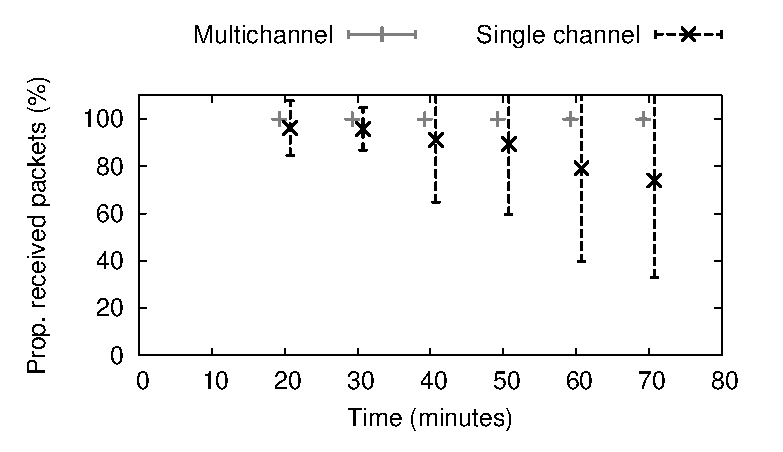
\includegraphics[width=0.45\textwidth]{experiments/mild.eps}}                
\subfigure[Moderate Interference]{\label{fig:mod}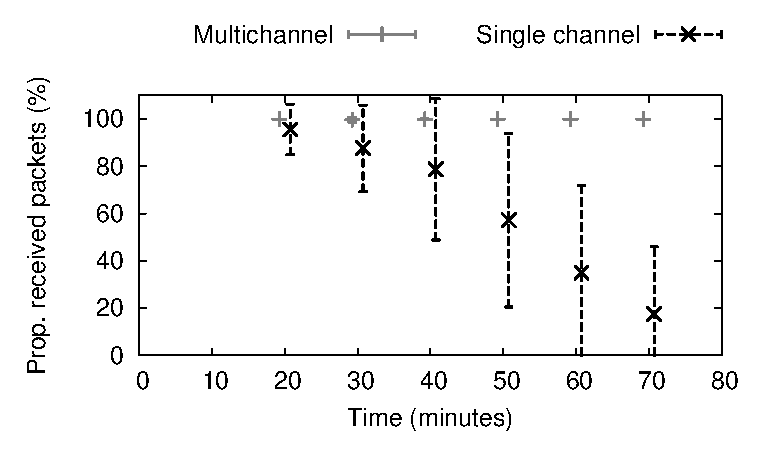
\includegraphics[width=0.45\textwidth]{experiments/moderate.eps}}
\subfigure[Extreme Interference]{\label{fig:extreme}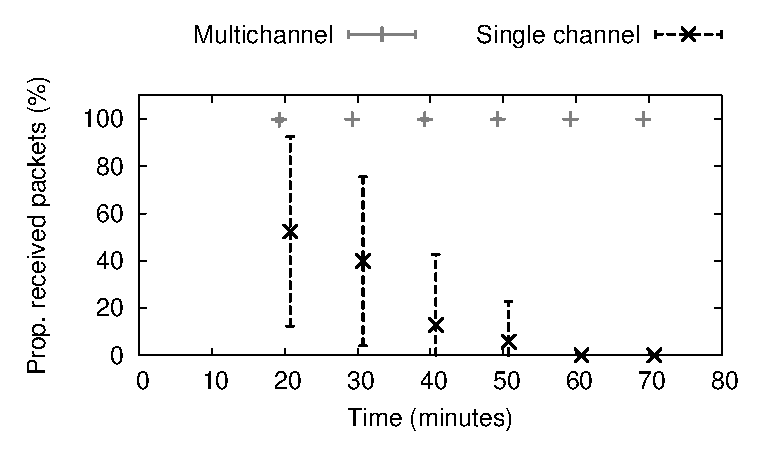
\includegraphics[width=0.45\textwidth]{experiments/extreme.eps}}
\caption{Level of packet loss for mild, moderate and extreme interference levels using single and multi-channel}
\label{fig:interference}
\end{figure}

We vary the interference rate, which is referred to as \emph{clear\textunderscore time} in \cite{Boano:2010:MSM:2127940.2127963} to 100\% (no interference), 75\% (mild), 50\% (moderate) and 25\% (extreme) where the percentage is the ratio of the time the channel is cleared from interference. The test is done to evaluate our protocol behaviour in different interference rate and to compare the result with a single channel case. Figure \ref{fig:interference} shows the mean results from ten simulation runs in each scenario and the error bars represent the standard deviation. We observed that during high interference and moderate interference, when the LPBR generates a random two hop channel for a node to change into, the receiving node will probe on the channel. It will either time out or the probing messages received are less than a threshold that allows for the node to change it's listening channel to the new channel. This is as expected as our protocol checks the channel each time before deciding on the new channel to avoid interference channel. By doing this, we can be sure that the node listening channel is a good channel. This enables us to use all available channels without blacklisting any channel until we are sure it is a bad channel through our probing process. The channel quality table is built at the LPBR that over time, can be used to learn good and bad channels based on several probing processes. 

In the mild interference case, all probing messages are received even though there are interference in that channel. This is because, the probing gives good result which means that the channel can be used. As the interference rate is mild, all packets are received. This is also the case with a single channel. The interference does not affect the transmissions as the interference is not frequent enough that enables the node to recover. However, the interference would slightly effect the packet transmission over time. We plan to run channel change processes periodically to avoid this from happening. %The tests were done using MiCMAC and CSMA. The nodes will check the channel, backoff and retransmit as necessary.

In the single channel,  the system cannot cope with the interference and as time goes on the RPL topology cannot continue to function sending and receiving packets. Figure \ref{fig:interference} shows that the rate of packet loss increases over time and when the interference is sufficient then packet reception will entirely stop sometimes within the first twenty minutes of the interference starting.  Figure \ref{fig:interference}(a) shows that the single channel model can cope but has degraded performance when the interference is mild, but when the interference becomes moderate then more than half the packets are lost towards the end of the simulation period.  When the interference is extreme, the packet loss increases to 100\% 
in all cases.

\subsection{Setup Overhead}
%//overhead?
%trickle - doubled each time but wait for a while so that it won't (affect?) with our protocol (sending messages; need to change channel which might be a problem?)

%//mention how much overhead there is agains RPL. 

%//say it is a one-off and compare it with data transmitted in one hour. packet transmitted high, overhead is negligible - real world, for low bit rate i.e video run for hours/months. "The.. is much smaller compared to the data period and during the data period the nodes can transmit multiple packets to do normal transmission"

%//mention that our protocol can transmit during the set up phase. so rpl set up forms the network then our protocol improves the network at a small cost in terms of messages and while leaving the network functional.

Obviously the system of changing channels and probing to see if a channel is free of interference introduces a certain amount of overhead into
the protocol.  This takes the form of (a) extra messages passed and (b) extra time taken to set up.  Default RPL on ContikiMAC for the topology considered in these experiments completed its set up using 276 packets.  Our multi-channel protocol completed its set up in 716 packets, that is an overhead of 440 packets on top of RPL. However, it is worth mentioning that this is a one-off cost.  This represents (in this experimental set up) approximately one hour of extra packets in the situation of a deployment that is meant to work for weeks or months.  In terms of set up time, our protocol begins to change channels only when the RPL set up process is complete (or at least stablises).  The set up time is 435 seconds beyond the 
RPL set up time of 286 seconds.  However, it should be noted that, in fact, our system remains fully functional and capable of sending packets during
the set up so this set up overhead does not matter to data transmission.


\section{Conclusion}
\label{sec:conclusion}
%//conclusion and future work

%//"Work is continuing to develop this protocol.  The next stages are 1) to improve the interference model in testing to a multiple channel interference model; 2) To move the implemenation to real hardware and 3) To allow continual updates on packet loss for each node so that channels can be changed dynamically when interference occurs."

We presented Multichannel RPL, a centralised cross layer channel change protocol as an extension to the existing RPL with ContikiMAC. Our protocol mitigates the effect of interference by avoiding the affected channel through probing when deciding a new channel. The results from the simulation show that our protocol avoided the interfered channel to maintain a high throughput over time. 

We are continuing with the work to further develop this protocol. The next stages that we plan to pursue is to improve the interference model that we used in testing to cover multiple channels interference. We plan to replicate the interference model to closely represent the real world where interference happen at many channels. We also plan to test our implementation on real hardware and to allow continual updates on packet loss for each node so that channels can be changed dynamically when interference occurs.

% The nature of our protocol that decides/run the decision making to the application layer gives us more opportunity to add the decision complexity - intelligence? and do real time channel checking. Our protocol maintains high reliability during heavily interfered periods where  ContikiMAC showed a low throughput of //////result?.



% conference papers do not normally have an appendix


% use section* for acknowledgement
\section*{Acknowledgment}
%The authors would like to thank...





% trigger a \newpage just before the given reference
% number - used to balance the columns on the last page
% adjust value as needed - may need to be readjusted if
% the document is modified later
%\IEEEtriggeratref{8}
% The "triggered" command can be changed if desired:
%\IEEEtriggercmd{\enlargethispage{-5in}}

% references section

% can use a bibliography generated by BibTeX as a .bbl file
% BibTeX documentation can be easily obtained at:
% http://www.ctan.org/tex-archive/biblio/bibtex/contrib/doc/
% The IEEEtran BibTeX style support page is at:
% http://www.michaelshell.org/tex/ieeetran/bibtex/
%\bibliographystyle{IEEEtran}
% argument is your BibTeX string definitions and bibliography database(s)
%\bibliography{IEEEabrv,../bib/paper}
%
% <OR> manually copy in the resultant .bbl file
% set second argument of \begin to the number of references
% (used to reserve space for the reference number labels box)
\label{references}
\nocite{*}
\bibliography{Bibliography}
\bibliographystyle{plain}
%\begin{thebibliography}{1}
%\input{Bibliography}
%\bibitem{IEEEhowto:kopka}
%H.~Kopka and P.~W. Daly, \emph{A Guide to \LaTeX}, 3rd~ed.\hskip 1em plus
%  0.5em minus 0.4em\relax Harlow, England: Addison-Wesley, 1999.

%\end{thebibliography}




% that's all folks
\end{document}


